\section{Experiments}

\subsection{Baselines}

We benchmark \ourmethod{} against two pipelines (App.~\ref{appendix:baseline_selection}): (1) a \textbf{Single Agent} baseline that processes all raw materials ($\mathcal{I}, \mathcal{E}, \mathcal{T}, \mathcal{G}, \mathcal{F}$) and executes end-to-end drafting and bibliography construction in a single LLM call, validating the necessity of a multi-agent system; and (2) \textbf{AI Scientist-v2}~\citep{yamada2025aiscientistv2}, a state-of-the-art system featuring multi-round citation gathering, VLM-guided plot refinement, and iterative self-reflection. To ensure fair comparison against baselines lacking diagram generation, we standardize visual inputs by restricting allowable figures to those extracted from ground-truth papers ($\mathcal{F} = \mathcal{F}_{GT}$). Furthermore, we adopt the \textit{sparse idea} as our standard setting to simulate realistic scenarios where researchers provide preliminary notes rather than mature formulations. To prevent pre-training data memorization, all evaluated writing pipelines employ a universal anti-leakage prompt (App.~\ref{appendix:info_leakage}).

\begin{figure}[tbp]
    \centering
    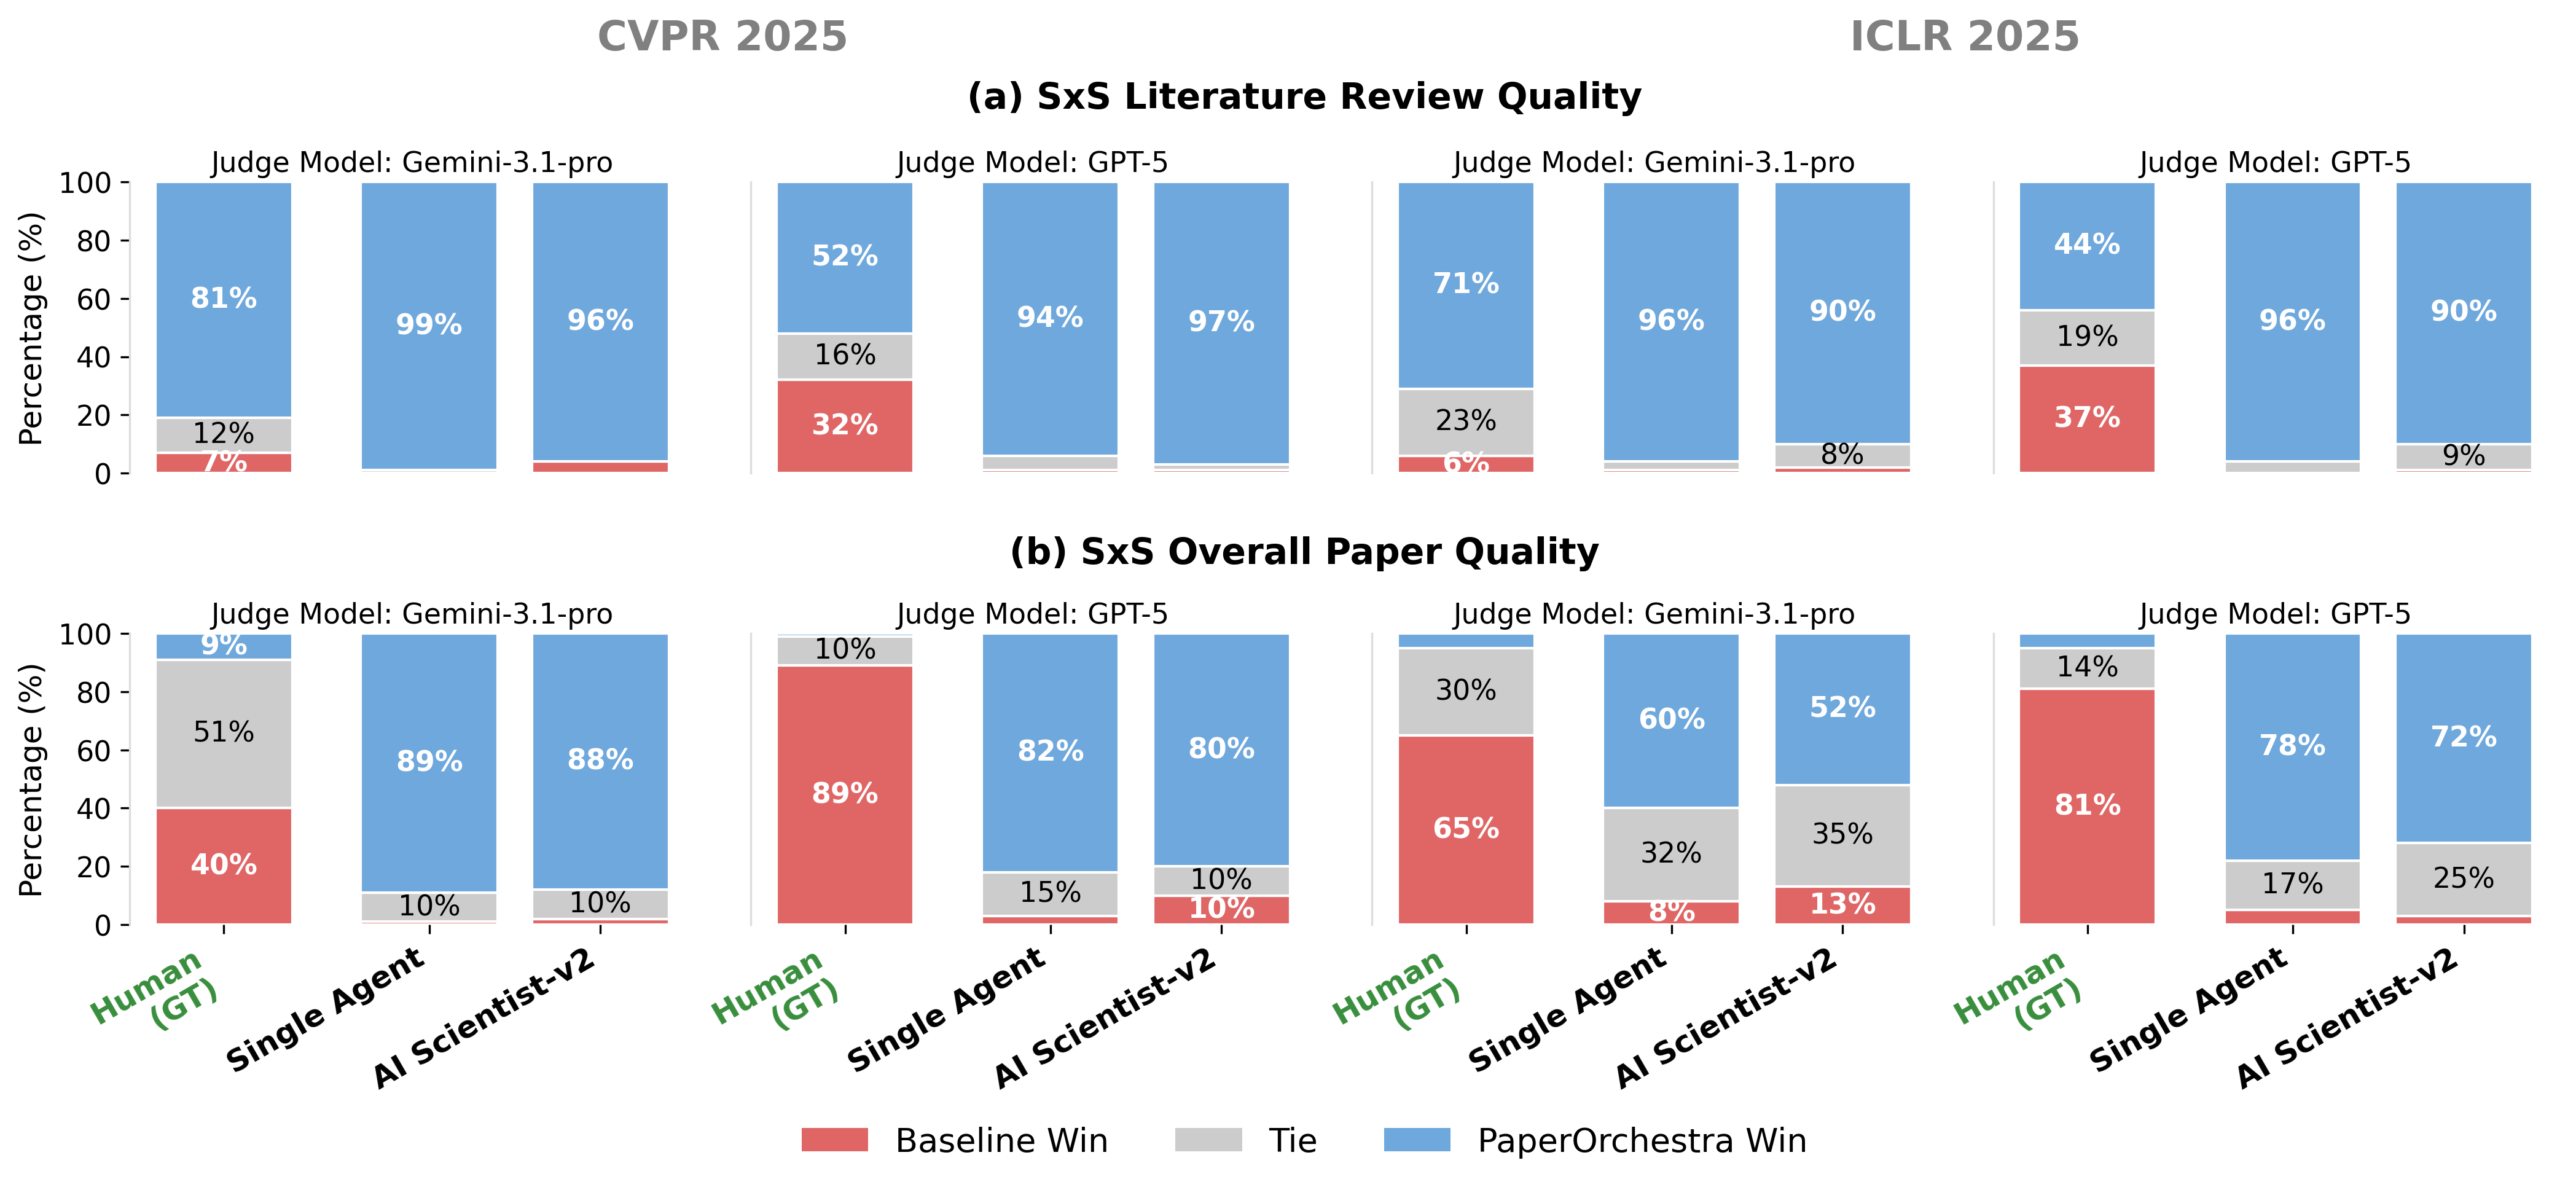
\includegraphics[width=\linewidth]{content/figures/sxs_merged_2x4_spaced.png} 
    \caption{Automated SxS evaluation of \ourmethod{} against baselines on the CVPR and ICLR 2025 datasets under the sparse idea setting. The \textbf{Human (GT)} baseline serves as an upper-bound reference. For both \textbf{(a)} literature review and \textbf{(b)} overall paper quality, \ourmethod{} significantly outperforms the AI baselines (Single Agent and AI Scientist-v2) across both judge models.}
    \label{fig:sxs_comparison}
\end{figure}

% ==========================================
% TABLE: Auto Reviewing System Results
% ==========================================
\begin{table}[tbp]
    \centering
    \resizebox{\textwidth}{!}{
    \begin{tabular}{llccccccccc}
        \toprule
        \textbf{Venue} & \textbf{Pipeline} & \begin{tabular}{@{}c@{}}\textbf{Originality} \\ \textbf{(1-4)}\end{tabular} & \begin{tabular}{@{}c@{}}\textbf{Quality} \\ \textbf{(1-4)}\end{tabular} & \begin{tabular}{@{}c@{}}\textbf{Clarity} \\ \textbf{(1-4)}\end{tabular} & \begin{tabular}{@{}c@{}}\textbf{Significance} \\ \textbf{(1-4)}\end{tabular} & \begin{tabular}{@{}c@{}}\textbf{Soundness} \\ \textbf{(1-4)}\end{tabular} & \begin{tabular}{@{}c@{}}\textbf{Presentation} \\ \textbf{(1-4)}\end{tabular} & \begin{tabular}{@{}c@{}}\textbf{Contribution} \\ \textbf{(1-4)}\end{tabular} & \begin{tabular}{@{}c@{}}\textbf{Overall} \\ \textbf{(1-10)}\end{tabular} & \begin{tabular}{@{}c@{}}\textbf{Acceptance} \\ \textbf{Rate (\%)}\end{tabular} \\
        \midrule
        \multicolumn{11}{c}{\cellcolor{gray!15}\textbf{AI Scientist-v2 Reviewer~\citep{yamada2025aiscientistv2}}} \\
        \midrule
        \multirow{4}{*}{CVPR 2025} 
        & Original (GT)   & 2.96 & \textbf{2.81} & \textbf{3.44} & \textbf{3.06} & \textbf{2.74} & \textbf{3.26} & \textbf{2.91} & \textbf{5.95} & \textbf{71.00} \\
        \cmidrule{2-11}
        & SingleAgent      & \cellcolor{best_color}\textbf{3.01} & 2.27 & 2.78 & \cellcolor{best_color}3.03 & 2.26 & 2.79 & \cellcolor{best_color}2.74 & 4.60 & 33.00 \\
        & AI Scientist-v2  & 2.93 & 2.11 & 2.80 & 2.85 & 2.15 & 2.82 & 2.61 & 4.22 & 22.00 \\
        & \ourmethod{}~(PlotOff)     & 2.95 & \cellcolor{best_color}2.43 & \cellcolor{best_color}3.40 & 2.97 & \cellcolor{best_color}2.42 & \cellcolor{best_color}3.22 & \cellcolor{best_color}2.74 & \cellcolor{best_color}5.12 & \cellcolor{best_color}48.00 \\
        \midrule
        \multirow{4}{*}{ICLR 2025} 
        & Original (GT)   & \textbf{2.99} & \textbf{2.79} & \textbf{3.41} & \textbf{3.03} & \textbf{2.76} & \textbf{3.30} & \textbf{2.94} & \textbf{5.81} & \textbf{63.00} \\
        \cmidrule{2-11}
        & SingleAgent     & \cellcolor{best_color}2.70 & 1.67 & 2.20 & 2.44 & 1.76 & 2.19 & 2.09 & 3.22 & 4.00 \\
        & AI Scientist-v2 & 2.58 & 1.76 & 2.27 & 2.46 & 1.82 & 2.29 & 2.16 & 3.42 & 11.00 \\
        & \ourmethod{}~(PlotOff)     & 2.68 & \cellcolor{best_color}2.10 & \cellcolor{best_color}2.82 & \cellcolor{best_color}2.57 & \cellcolor{best_color}2.12 & \cellcolor{best_color}2.79 & \cellcolor{best_color}2.37 & \cellcolor{best_color}4.10 & \cellcolor{best_color}22.00 \\
        \midrule
        \multicolumn{11}{c}{\cellcolor{gray!15}\textbf{ScholarPeer Reviewer~\citep{goyal2026scholarpeer}}} \\
        \midrule
        \multirow{4}{*}{CVPR 2025} 
        & Original (GT)   & \textbf{3.22} & \textbf{3.02} & 3.54 & \textbf{3.63} & 2.87 & 3.39 & \textbf{3.42} & \textbf{7.07} & \textbf{86.00} \\
        \cmidrule{2-11}
        & SingleAgent     & \cellcolor{best_color}\textbf{3.22} & 2.79 & 3.46 & 3.48 & 2.72 & 3.34 & 3.29 & 6.35 & 71.00 \\
        & AI Scientist-v2 & 3.11 & 2.71 & 3.44 & 3.39 & 2.64 & 3.37 & 3.22 & 6.30 & 70.00 \\
        & \ourmethod{}~(PlotOff)  & 3.13 & \cellcolor{best_color}2.95 & \cellcolor{best_color}\textbf{3.75} & \cellcolor{best_color}3.56 & \cellcolor{best_color}\textbf{2.91} & \cellcolor{best_color}\textbf{3.64} & \cellcolor{best_color}3.34 & \cellcolor{best_color}6.93 & \cellcolor{best_color}84.00 \\
        \midrule
        \multirow{4}{*}{ICLR 2025} 
        & Original (GT)   & \textbf{3.33} & \textbf{3.14} & \textbf{3.76} & \textbf{3.74} & \textbf{3.05} & \textbf{3.59} & \textbf{3.57} & \textbf{7.48} & \textbf{94.00} \\
        \cmidrule{2-11}
        & SingleAgent     & 3.26 & 2.73 & 3.27 & 3.48 & 2.71 & 3.20 & 3.25 & 6.35 & 72.00 \\
        & AI Scientist-v2 & 3.23 & 2.62 & 3.28 & 3.41 & 2.60 & 3.23 & 3.11 & 6.04 & 64.00 \\
        & \ourmethod{}~(PlotOff)     & \cellcolor{best_color}3.35 & \cellcolor{best_color}2.96 & \cellcolor{best_color}3.65 &\cellcolor{best_color}3.59 & \cellcolor{best_color}2.94 & \cellcolor{best_color}3.48 & \cellcolor{best_color}3.37 & \cellcolor{best_color}7.03 & \cellcolor{best_color}81.00 \\
        \bottomrule
    \end{tabular}
    }
  \caption{Holistic technical quality evaluation via the AI Scientist-v2~\citep{yamada2025aiscientistv2} and ScholarPeer~\citep{goyal2026scholarpeer} frameworks (Sparse Idea Setting). Higher scores indicate better manuscript quality and higher simulated acceptance rates. \textbf{Bold} indicates best scores; while \colorbox{best_color}{green} highlights the highest score achieved by an AI pipeline.}
  \label{tab:combined_reviewer_quality}
\end{table}
\subsection{Autoraters}
% We evaluate the generated manuscripts using four automatic rating systems. 

\paragraph{Citation F1.} To quantitatively assess citation coverage, we compare the generated reference list against the ground-truth (GT) paper. Using an LLM provided with the paper context (see App.~\ref{appendix:autorater_prompts}), we partition the GT references into two categories: (1) \textbf{P0 (Must-Cite)} comprises core citations strictly necessary for contextualizing the work, including direct experimental baselines, utilized datasets, metrics, and foundational methodologies upon which the paper directly builds; (2) \textbf{P1 (Good-to-Cite)} includes all remaining GT citations, providing valuable but non-essential background context such as orthogonal work or supplementary information. To ensure accurate matching, we extract reference lists from both the GT and generated papers and resolve them to unique entity IDs using the Semantic Scholar API. We then compute Precision, Recall, and F1 scores independently for the P0 set, the P1 set, and the combined overall reference set.

\paragraph{Literature Review Quality.} To qualitatively evaluate the generated \textit{Introduction} and \textit{Related Work} sections, we employ an LLM evaluator (App.~\ref{appendix:autorater_prompts}) to score the generated text from 0--100 across six axes: coverage and completeness, relevance and focus, critical analysis and synthesis, positioning and novelty, organization, and citation rigor. To mitigate standard LLM score inflation, the evaluation is grounded against venue-specific average citation counts. The system enforces strict score caps and penalties for purely descriptive summaries, unsupported novelty claims, or citation padding, outputting an overall quality score for each paper.

\paragraph{Overall Quality.} To evaluate the holistic technical quality of the generated papers, we employ two AI-based peer review frameworks simulating expert assessment: (1) the \textbf{AI Scientist-v2 Reviewer}~\citep{yamada2025aiscientistv2}, an automated module for structured manuscript evaluation; and (2) \textbf{ScholarPeer}~\citep{goyal2026scholarpeer}, a search-enabled multi-agent system mimicking expert workflows via iterative retrieval and evidence checking. Both systems yield multi-axis scores, an overall rating, and a simulated acceptance decision.

\paragraph{Side-by-Side (SxS) Comparison.} To directly compare manuscripts generated from the same research idea across different pipelines, we implement two automated SxS LLM evaluators. \textbf{(1) SxS Literature Review Quality} extracts the \textit{Introduction} and \textit{Related Work} to assess problem framing, prior work coverage, organization and synthesis, contribution positioning, and readability. \textbf{(2) SxS Paper Quality} holistically compares the full manuscript (including visual layout) across six axes: scientific depth, technical execution, logical flow, writing clarity, presentation of evidence, and academic style. To mitigate LLM positional bias, we evaluate each pair of manuscripts in both orderings. The final aggregated outcome is recorded as a \textit{win} (two wins, or one win and one tie), a \textit{tie} (one win and one loss, or two ties), or a \textit{loss}.

\subsection{Results}
\paragraph{Side-by-Side Comparison.} As shown in \Cref{fig:sxs_comparison}, \ourmethod{} consistently outperforms both the Single Agent baseline and AI Scientist-v2 in SxS evaluations. In \textit{Literature Review Quality}, our framework dominates the autonomous baselines, achieving absolute win margins of \textbf{88\%--99\%}. For \textit{Overall Paper Quality}, although Human (GT) remains the upper bound, \ourmethod{} substantially surpasses all tested AI competitors. It strongly outperforms AI Scientist-v2 and the Single Agent by margins of \textbf{39\%--86\%} and \textbf{52\%--88\%}, respectively, across all settings, confirming that our multi-agent architecture significantly enhances overall manuscript quality (cost analysis in App.~\ref{appendix:cost}).

\paragraph{Technical Quality.} As detailed in \Cref{tab:combined_reviewer_quality}, we evaluate holistic manuscript quality using the AI Scientist-v2 and ScholarPeer frameworks. Under ScholarPeer, \ourmethod{} achieves high simulated acceptance rates of \textbf{84\%} (CVPR) and \textbf{81\%} (ICLR), closely tracking Human (GT) baselines (\textbf{86\%} and \textbf{94\%}, respectively). It significantly outperforms existing AI pipelines, delivering absolute acceptance gains of \textbf{13\%} (CVPR) and \textbf{9\%} (ICLR) over the strongest autonomous baseline. Beyond acceptance rates, \ourmethod{} dominates across critical sub-axes (notably \textit{Clarity}, \textit{Presentation}, and \textit{Soundness}), demonstrating that our multi-agent system yields structurally coherent and technically sound manuscripts.


% ==========================================
% TABLE: Citation F1 Quality
% ==========================================
\begin{table}[tbp]
    \centering
    \resizebox{\textwidth}{!}{%
    \begin{tabular}{ll c c ccc ccc}
        \toprule
        \multirow{2}{*}{\textbf{Venue}} & \multirow{2}{*}{\textbf{Pipeline}} & \multirow{2}{*}{\begin{tabular}{@{}c@{}}\textbf{GT Avg} \\ \textbf{\# Cites}\end{tabular}} & \multirow{2}{*}{\begin{tabular}{@{}c@{}}\textbf{Avg} \\ \textbf{\# Cites}\end{tabular}} & \multicolumn{3}{c}{\textbf{Gemini-3.1-Pro}} & \multicolumn{3}{c}{\textbf{GPT5}} \\
        \cmidrule(lr){5-7} \cmidrule(lr){8-10}
        & & & & \begin{tabular}{@{}c@{}}\textbf{Overall} \\ \textbf{F1}\end{tabular} & \begin{tabular}{@{}c@{}}\textbf{P0} \\ \textbf{Recall}\end{tabular} & \begin{tabular}{@{}c@{}}\textbf{P1} \\ \textbf{Recall}\end{tabular} & \begin{tabular}{@{}c@{}}\textbf{Overall} \\ \textbf{F1}\end{tabular} & \begin{tabular}{@{}c@{}}\textbf{P0} \\ \textbf{Recall }\end{tabular} & \begin{tabular}{@{}c@{}}\textbf{P1} \\ \textbf{Recall}\end{tabular} \\
        \midrule
        \multirow{3}{*}{CVPR 2025} 
        & SingleAgent      & \multirow{3}{*}{58.52} & 11.46 & 28.03 & 60.84 & 2.77 & 28.16 & 63.04 & 3.27 \\
        & AI Scientist-v2  & & 14.18 & 17.15 & 36.12 & 3.26 & 17.26 & 37.46 &  3.30 \\
        & \ourmethod{} (PlotOff)     & & \cellcolor{best_color}47.98 & \cellcolor{best_color}\textbf{29.65} & \cellcolor{best_color}\textbf{63.58} & \cellcolor{best_color}\textbf{15.85} & \cellcolor{best_color}\textbf{29.92} & \cellcolor{best_color}\textbf{65.17} & \cellcolor{best_color}\textbf{16.43} \\
        \midrule
        \multirow{3}{*}{ICLR 2025} 
        & SingleAgent      & \multirow{3}{*}{59.18} & 9.75 & 23.16 & 48.41 & 3.09 & 23.29 & 50.75 & 3.23 \\
        & AI Scientist-v2  & & 13.71 & 15.80 & 33.66 & 3.07 & 15.94 & 34.73 & 3.36  \\
        & \ourmethod{} (PlotOff)     & & \cellcolor{best_color}45.73 & \cellcolor{best_color}\textbf{27.76} & \cellcolor{best_color}\textbf{54.48} & \cellcolor{best_color}\textbf{16.43} & \cellcolor{best_color}\textbf{27.97} & \cellcolor{best_color}\textbf{55.70} & \cellcolor{best_color}\textbf{17.11} \\
        \bottomrule
    \end{tabular}%
    } % End of resizebox
    \caption{Citation F1 evaluation (Sparse Idea Setting). P0 and P1 denote must-cite and good-to-cite references, respectively. F1 and Recall are percentages.}
    \label{tab:citation_f1}
\end{table}
% ==========================================
% TABLE: Literature Review Quality (Double Column)
% ==========================================
\begin{table*}[tbp]
    \centering
    \resizebox{\textwidth}{!}{
    \begin{tabular}{llccccccc}
        \toprule
        \multirow{2}{*}{\textbf{Venue}} & \multirow{2}{*}{\textbf{Pipeline}} & \textbf{Citation} & \textbf{Coverage \&} & \textbf{Critical Analysis} & \textbf{Organization} & \textbf{Positioning} & \textbf{Relevance} & \textbf{Overall} \\
        & & \textbf{Practices} & \textbf{Completeness} & \textbf{\& Synthesis} & \textbf{\& Writing} & \textbf{\& Novelty} & \textbf{\& Focus} & \textbf{Score} \\
        \midrule
        \multicolumn{9}{c}{{\cellcolor{gray!15}\textit{Judge Model: Gemini-3.1-Pro}}} \\
        \midrule
        \multirow{4}{*}{CVPR 2025} 
        & Human (GT)   & 69.88 & \textbf{71.55} & 65.80 & 74.31 & 75.55 & 78.25 & 71.08 \\
        \cmidrule{2-9}
        & SingleAgent     & 36.83 & 30.10 & 52.93 & 77.03 & 66.45 & 71.40 & 43.04 \\
        & AI Scientist-v2 & 39.24 & 34.25 & 54.83 & 77.21 & 65.16 & 69.12 & 45.43 \\
        & \ourmethod{} (PlotOff)     & \cellcolor{best_color}\textbf{75.36} & \cellcolor{best_color}70.15 & \cellcolor{best_color}\textbf{79.01} & \cellcolor{best_color}\textbf{83.74} & \cellcolor{best_color}\textbf{82.68} & \cellcolor{best_color}\textbf{81.15} & \cellcolor{best_color}\textbf{78.30} \\
        \midrule
        \multirow{4}{*}{ICLR 2025} 
        & Human (GT)   & \textbf{71.66} & \textbf{68.30} & 74.60 & 80.54 & \textbf{82.22} & \textbf{80.67} & 75.18 \\
        \cmidrule{2-9}
        & SingleAgent     & 33.03 & 26.35 & 49.80 & 75.38 & 61.14 & 69.70 & 38.91 \\
        & AI Scientist-v2 & 37.60 &  32.27 & 51.84 & 75.74 & 62.96 & 67.20 & 42.98 \\
        & \ourmethod{} (PlotOff)     & \cellcolor{best_color}71.15 & \cellcolor{best_color}65.71 & \cellcolor{best_color}\textbf{77.34} & \cellcolor{best_color}\textbf{82.02} & \cellcolor{best_color}81.94 & \cellcolor{best_color}80.08 & \cellcolor{best_color}\textbf{76.23} \\
        \midrule
        \multicolumn{9}{c}{{\cellcolor{gray!15}\textit{Judge Model: GPT5}}} \\
        \midrule
        \multirow{4}{*}{CVPR 2025} 
        & Human (GT)   & 63.47 & 63.86 & 57.36 & 76.16 & \textbf{61.34} & \textbf{73.23} & 53.66 \\
        \cmidrule{2-9}
        & SingleAgent     & 49.69 & 47.01 & 54.49 & 76.55 & 56.62 & 70.60 & 44.33 \\
        & AI Scientist-v2 & 49.18 & 47.59 & 53.71 & 75.71 & 55.80 & 69.00 & 43.57 \\
        & \ourmethod{} (PlotOff)     & \cellcolor{best_color}\textbf{63.88} & \cellcolor{best_color}\textbf{64.13} & \cellcolor{best_color}\textbf{60.04} & \cellcolor{best_color}\textbf{77.46} & \cellcolor{best_color}59.18 & \cellcolor{best_color}72.65 & \cellcolor{best_color}\textbf{53.99} \\
        \midrule
        \multirow{4}{*}{ICLR 2025} 
        & Human (GT)   & 61.61 & 60.91 & 58.75 & 77.19 & \textbf{62.91} & 73.11 & \textbf{55.53} \\
        \cmidrule{2-9}
        & SingleAgent     & 49.34 & 45.97 & 54.10 & 77.79 & 56.47 & 71.52 & 44.30 \\
        & AI Scientist-v2 & 49.55 & 48.26 & 54.18 & 76.62 & 56.08 & 69.86 & 44.29 \\
        & \ourmethod{} (PlotOff)     & \cellcolor{best_color}\textbf{62.54} & \cellcolor{best_color}\textbf{62.12} & \cellcolor{best_color}\textbf{60.58} & \cellcolor{best_color}\textbf{78.70} & \cellcolor{best_color}60.21& \cellcolor{best_color}\textbf{73.58} & \cellcolor{best_color}54.15 \\
        \bottomrule
    \end{tabular}
    }
    \caption{Literature review quality assessed by LLM-as-a-Judge (0--100 scale, Sparse Idea Setting). All numbers are percentages.}
    \label{tab:lit_review_quality}
\end{table*}

\paragraph{Citation Coverage.} \Cref{tab:citation_f1} demonstrates \ourmethod{} successfully mitigates under-citation issues. While autonomous baselines achieve competitive Overall F1 scores, this is a mathematical artifact of their extremely low citation counts (averaging 9--14). They focus on fetching obvious P0 papers, which inflates their F1 scores but leaves P1 Recall near zero. In contrast, our framework generates \textbf{45.73--47.98} citations, closely mirroring Human (GT) writeups ($\sim$59). Alongside improving P0 Recall by absolute margins of \textbf{2.13\%--6.07\%}, \ourmethod{} significantly increases P1 Recall by \textbf{12.59\%--13.75\%} over the strongest baselines. This proves our method actively explores the broader academic landscape rather than relying on shallow keyword matching.

\paragraph{Literature Review Quality.} Citation F1 alone cannot fully evaluate literature synthesis; a review must also identify gaps and motivate the proposed method. From \Cref{tab:lit_review_quality}, \ourmethod{} achieves absolute Overall Score gains of \textbf{32.87\%--33.25\%} (Gemini-3.1-Pro) and \textbf{9.66\%--9.85\%} (GPT-5) over the strongest AI baseline, remaining highly comparable to Human baselines. Dominating in \textit{Citation Practices} and \textit{Critical Analysis}, our framework synthesizes analytical, well-grounded narratives rather than generic LLM summaries.


\subsection{Human Evaluation}

% ==========================================
% Side-by-Side Figure and Correlation Table
% ==========================================
\begin{figure}[tbp]
    \centering
    
    % Left Side: The Bar Chart (Subfigure a)
    \begin{subfigure}[b]{0.58\textwidth}
        \centering
        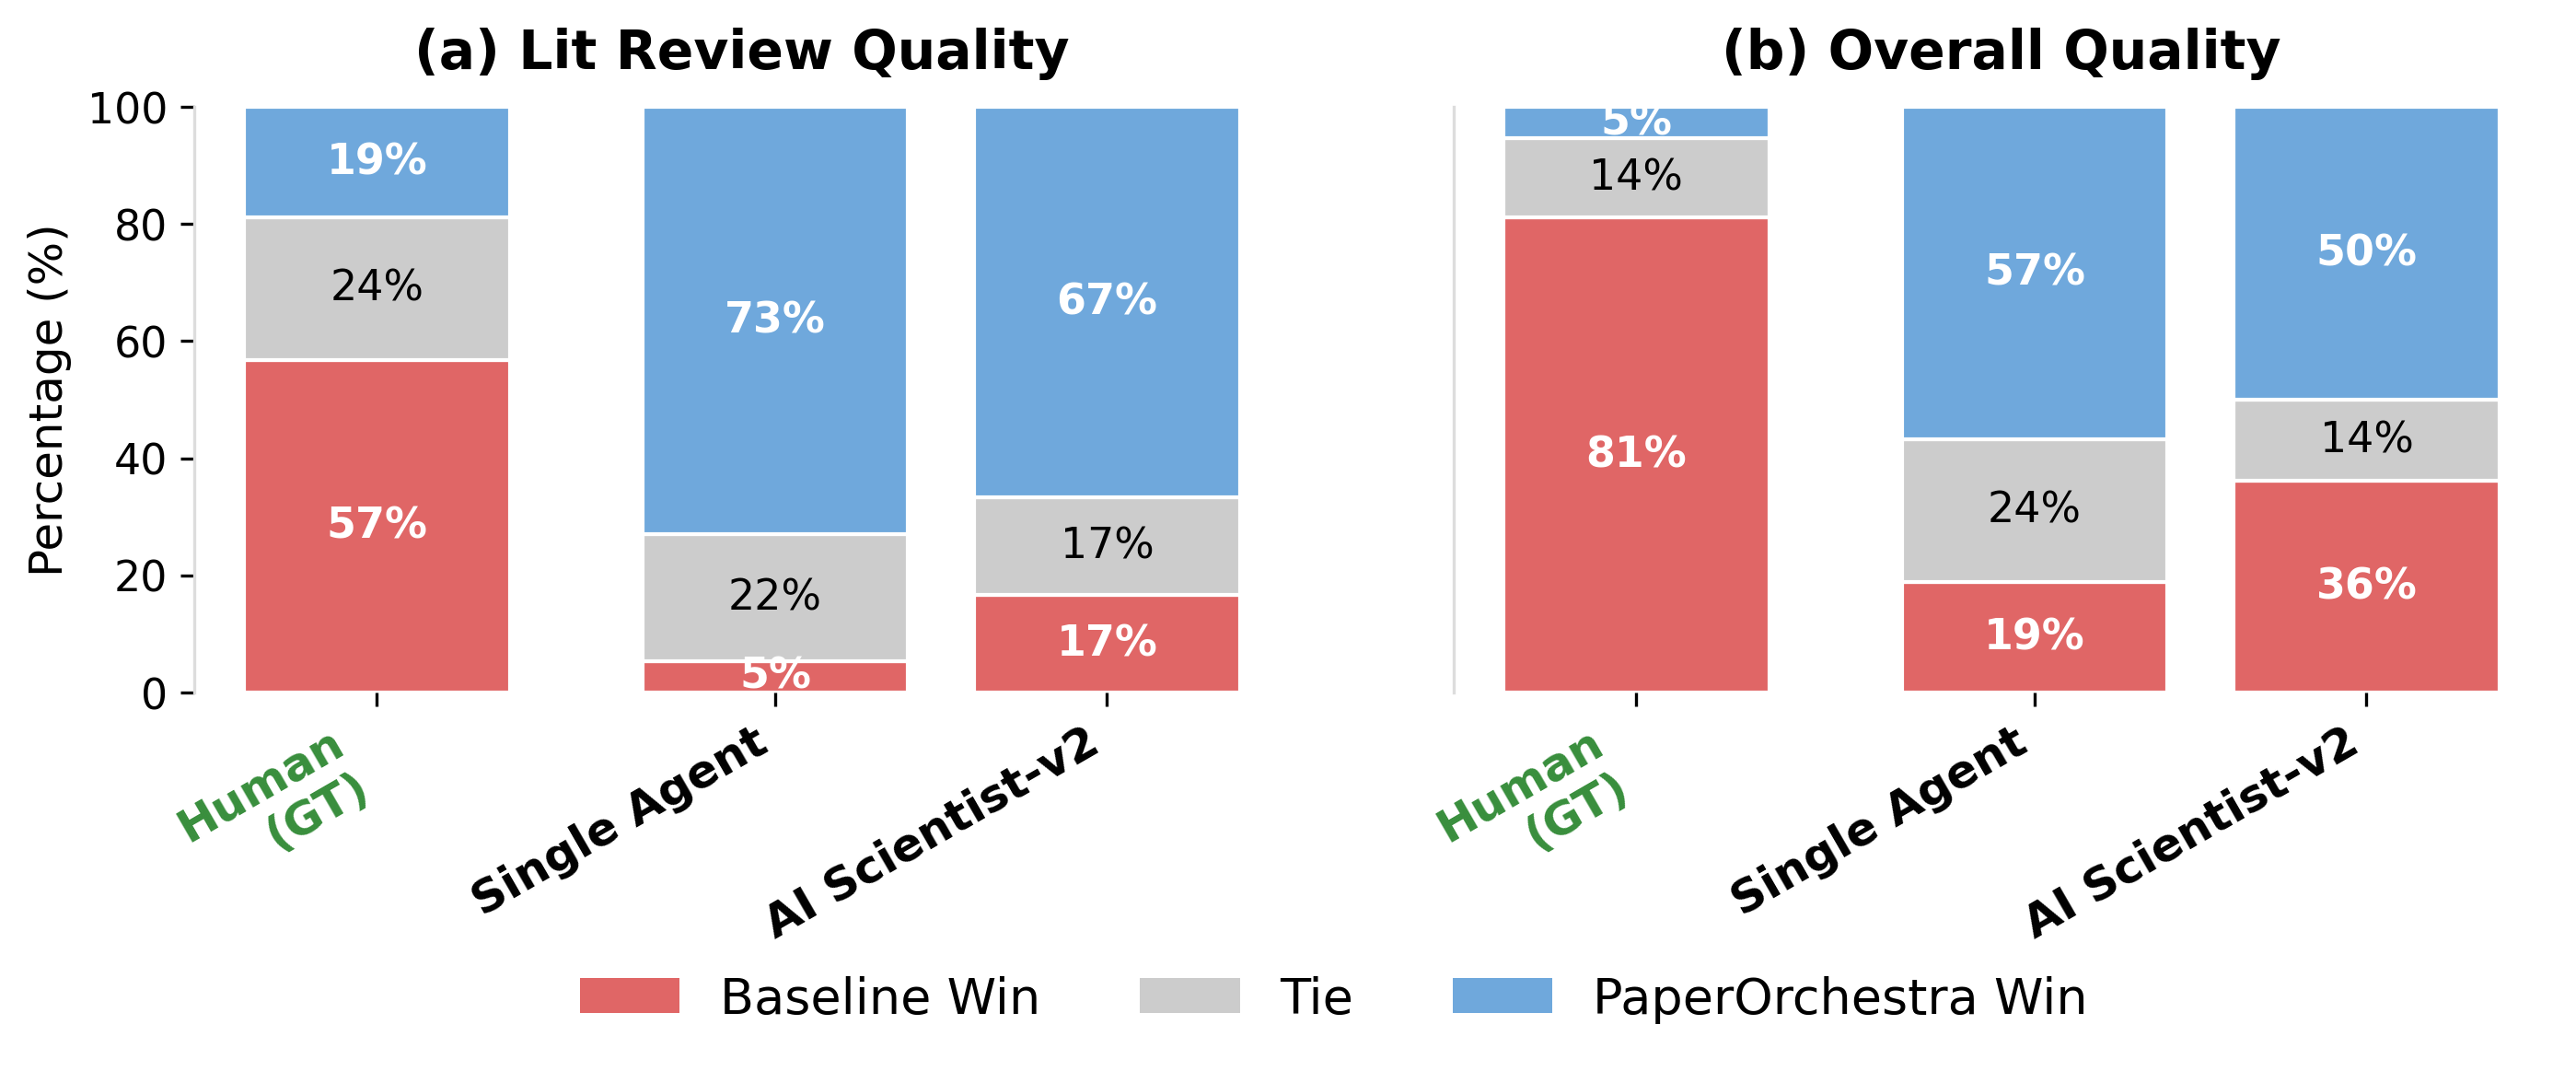
\includegraphics[width=\linewidth]{content/figures/human_eval_bar.png}
        \caption{Human SxS Evaluation Results}
        \label{fig:human_sxs_a}
    \end{subfigure}
    \hfill
    % Right Side: The Correlation Table (Subfigure b)
    \begin{subfigure}[b]{0.4\textwidth}
        \centering
        \resizebox{\linewidth}{!}{%
        \begin{tabular}{llcc}
            \toprule
            \textbf{Metric} & \textbf{Judge(s)} & \textbf{Pearson} & \textbf{Spearman} \\
            \midrule
            \multicolumn{4}{c}{\cellcolor{gray!15}\textit{Human vs. Autorater Correlation}} \\
            \midrule
            \multirow{2}{*}{Lit Review Quality} 
            & Gemini-3.1-Pro & 0.0868 & 0.0715 \\
            & GPT-5 & \textbf{0.2764} & \textbf{0.2300} \\
            \midrule
            \multirow{2}{*}{Overall Quality} 
            & Gemini-3.1-Pro & 0.5672 & 0.5727 \\
            & GPT-5 & \textbf{0.6458} & \textbf{0.6355} \\
            \midrule
            \multicolumn{4}{c}{\cellcolor{gray!15}\textit{Inter-Autorater Correlation (Gemini-3.1-Pro vs. GPT-5)}} \\
            \midrule
            Lit Review Quality & \multicolumn{1}{c}{--} & 0.5697 & 0.5615 \\
            Overall Quality & \multicolumn{1}{c}{--} & \textbf{0.7395} & \textbf{0.7454} \\
            \bottomrule
        \end{tabular}%
        }
        \vspace{0.5em} % Reduced vertical padding since the table is taller now
        \caption{Autorater Validation Metrics}
        \label{fig:autorater_correlation_b}
    \end{subfigure}
    
    \caption{Human \& Autorater Evaluation (Sparse Idea Setting). \textbf{(a)} Human preferences for \ourmethod{} vs.\ baselines. \textbf{(b)} GPT-5 strongly correlates with human scores on overall quality, alongside high inter-autorater consistency between distinct LLM judges.}
    \label{fig:human_eval_combined}
\end{figure}

To validate automated SxS metrics and assess human-perceived manuscript quality, we recruited 11 AI researchers to evaluate 40 randomly sampled papers (20 per venue) from \ourdataset{}. For each paper, \ourmethod{} was compared against all baselines (Human GT, Single Agent, and AI Scientist-v2), yielding 180 paired evaluations (App.~\ref{appendix:human_eval}).

Human preferences correlate strongly with our GPT-5 evaluator for Overall Quality (Pearson $r=0.6458$, Spearman $\rho=0.6355$; Figure~\ref{fig:autorater_correlation_b}). Literature review correlation is lower due to inherent LLM self-bias. Manual inspection reveals LLMs tend to act as structural graders, rewarding rigid formatting such as explicit "Problem-Gap-Solution" paragraphs or bulleted thematic groups. In contrast, human experts prioritize dense, pragmatic factuality and a nuanced, narrative-driven flow, which the autorater often mistakenly penalizes for lacking explicit formatting cues. Nevertheless, relative rankings remain strictly consistent. The stability of our automated SxS metrics is further validated by high inter-autorater agreement across different LLM judges (Figure~\ref{fig:autorater_correlation_b}). Human SxS evaluations (Figure~\ref{fig:human_sxs_a}) confirm \ourmethod{} strongly outperforms AI baselines by absolute margins of \textbf{50\%--68\%} (Literature Review) and \textbf{14\%--38\%} (Overall Quality). It also achieves a highly competitive \textbf{43\%} tie/win rate against human GT in literature synthesis. 


\subsection{Ablation Studies}

\begin{table}[tbp]
    \centering
    \resizebox{0.8\linewidth}{!}{%
    \begin{tabular}{ll ccc c ccc}
        \toprule
        \multirow{2}{*}{\textbf{Venue}} & \multirow{2}{*}{\textbf{Metric}} & \multicolumn{3}{c}{\textbf{Gemini-3.1-Pro}} && \multicolumn{3}{c}{\textbf{GPT-5}} \\
        \cmidrule{3-5} \cmidrule{7-9}
        & & \textbf{Sparse Win} & \textbf{Tie} & \textbf{Dense Win} && \textbf{Sparse Win} & \textbf{Tie} & \textbf{Dense Win} \\
        \midrule
        \multirow{2}{*}{CVPR 2025} 
        & Paper Quality & 18\% & 26\% & \cellcolor{best_color}56\% && 24\% & 32\% & \cellcolor{best_color}44\% \\
        & Lit Review    & 37\% & 24\% & \cellcolor{best_color}39\% && \cellcolor{best_color}40\% & 22\% & 38\% \\
        \midrule
        \multirow{2}{*}{ICLR 2025} 
        & Paper Quality & 24\% & 31\% & \cellcolor{best_color}45\% && 20\% & 37\% & \cellcolor{best_color}43\% \\
        & Lit Review    & 33\% & 33\% & \cellcolor{best_color}34\% && \cellcolor{best_color}32\% & 40\% & 28\% \\
        \bottomrule
    \end{tabular}%
    }
    \caption{Automated SxS evaluation of Sparse vs.\ Dense idea settings.}
    \label{tab:ablation_sparse_dense}
\end{table}
\begin{table}[tbp]
    \centering
    \resizebox{0.8\linewidth}{!}{%
    \begin{tabular}{l ccc c ccc}
        \toprule
        \multirow{2}{*}{\textbf{Venue}} & \multicolumn{3}{c}{\textbf{Gemini-3.1-Pro}} && \multicolumn{3}{c}{\textbf{GPT-5}} \\
        \cmidrule{2-4} \cmidrule{6-8}
        & \textbf{PlotOff Win} & \textbf{Tie} & \textbf{PlotOn Win} && \textbf{PlotOff Win} & \textbf{Tie} & \textbf{PlotOn Win} \\
        \midrule
        CVPR 2025 & \cellcolor{best_color}34\% & 32\% & 34\% && \cellcolor{best_color}49\% & 19\% & 32\% \\
        ICLR 2025 & \cellcolor{best_color}35\% & 37\% & 28\% && \cellcolor{best_color}36\% & 38\% & 26\% \\
        \bottomrule
    \end{tabular}%
    }
    \caption{Automated SxS Paper Quality evaluating the Plotting Agent. Despite lacking access to data represented by GT visuals, \textit{PlotOn} achieves highly competitive performance against \textit{PlotOff} that use human-authored figures.}
    \label{tab:ablation_plotting}
\end{table}

\paragraph{Sparse vs.\ Dense Idea}
\Cref{tab:ablation_sparse_dense} evaluates the impact of input density. For \textit{Overall Paper Quality}, the Dense idea setting dominates win rates (\textbf{43\%--56\%} vs.\ \textbf{18\%--24\%}) by facilitating more rigorous methodology generation. Meanwhile, \textit{Literature Review Quality} exhibits near-parity, with the Sparse setting securing \textbf{32\%--40\%} against Dense's \textbf{28\%--39\%}. This demonstrates the exceptional robustness of \ourmethod: our \textit{Literature Review Agent} autonomously executes targeted searches and identifies research gaps without relying heavily on the dense input drafted by human. Additional qualitative comparisons are provided in App.~\ref{appendix:paper_viz_sparse_dense}.

\paragraph{Autonomous Visual Generation (PlotOff vs.\ PlotOn)}
\Cref{tab:ablation_plotting} evaluates our \textit{Plotting Agent} by comparing papers using human-authored GT figures (\textit{PlotOff}) vs. autonomously generated visuals (\textit{PlotOn}). Although \textit{PlotOff} benefits from an inherent information advantage (GT figures often embed supplementary results absent from raw input logs), \textit{PlotOn} remains highly competitive, securing ties or wins in \textbf{51\%--66\%} of SxS matchups across all four setups. As shown in App.~\ref{appendix:paper_viz_sxs}, \ourmethod{} synthesizes coherent visuals from scratch, effectively augmenting the manuscript and reinforcing the scientific narrative.

\begin{figure}[tbp]
    \centering    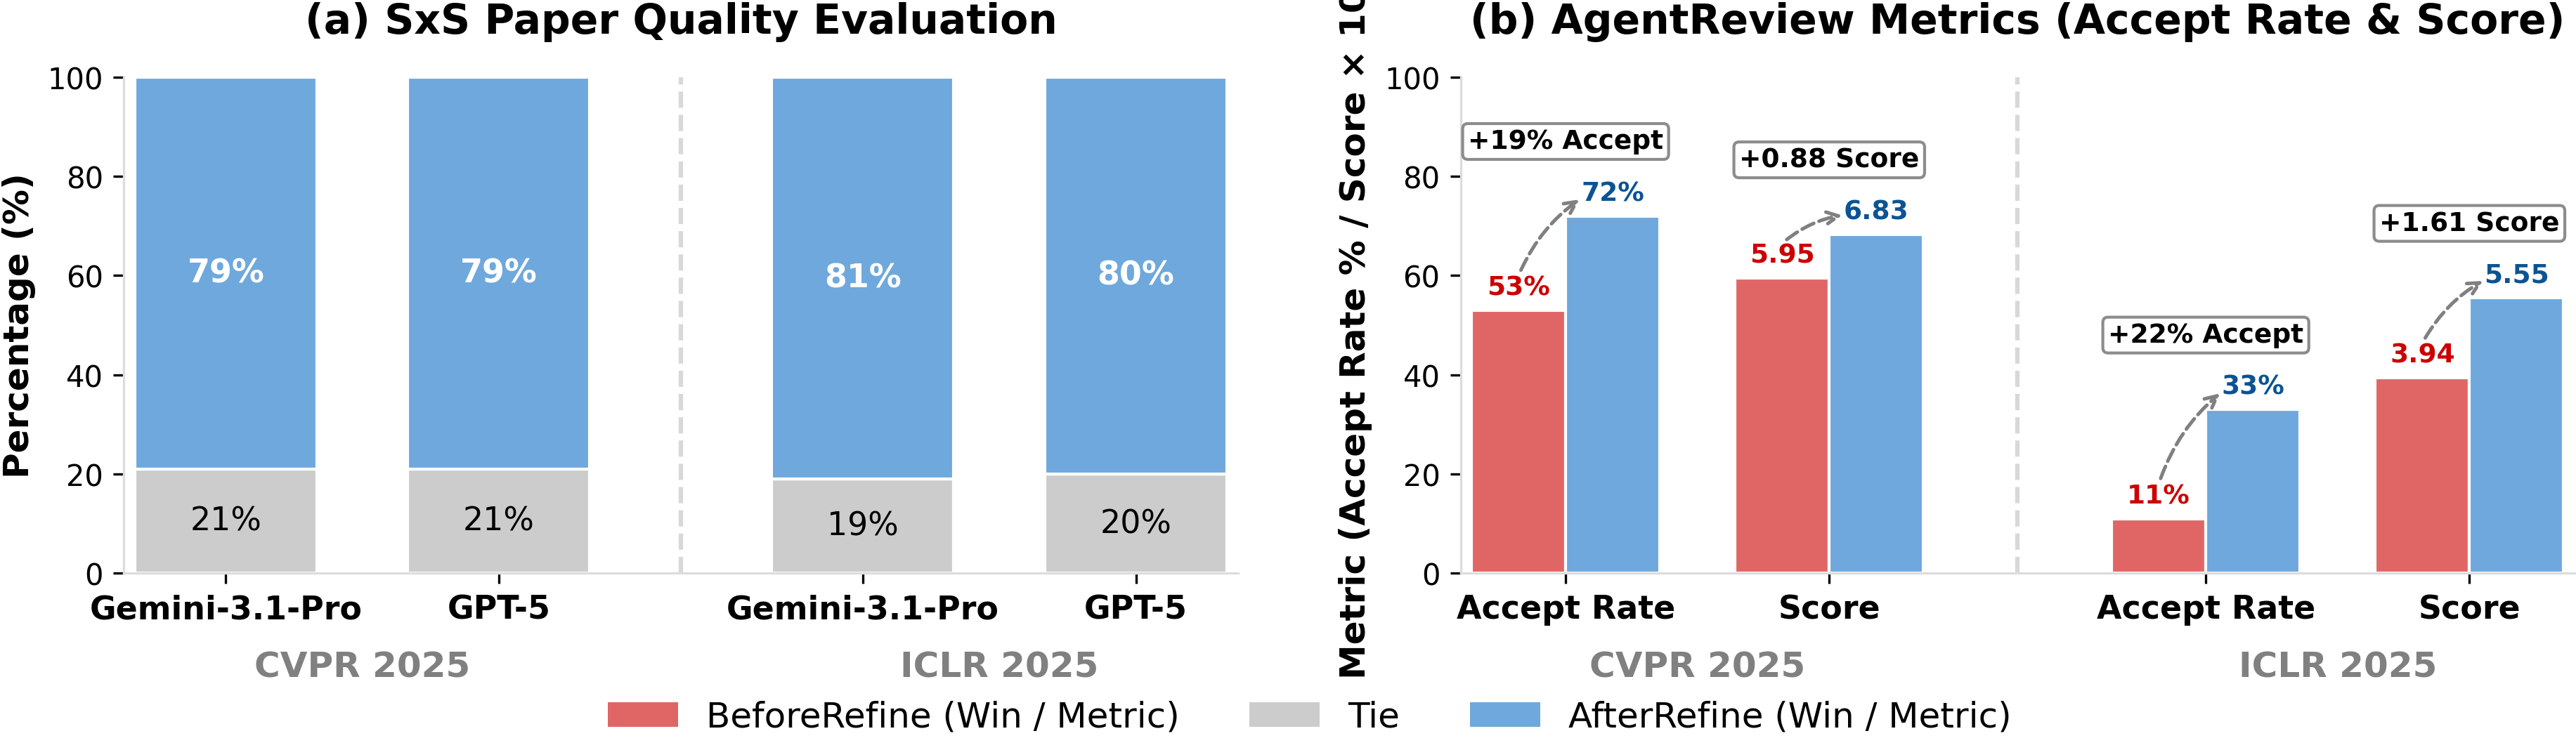
\includegraphics[width=\linewidth]{content/figures/ablation_refinement.png}
    \caption{\textbf{Impact of the Content Refinement Agent.} (a) In automated SxS paper quality evaluation, refined manuscripts dominates. (b) This improvement is reflected through absolute gains in acceptance rates simulated by AgentReview~\citep{jin2024agentreview}.}
    \label{fig:ablation_refinement}
\end{figure}

\paragraph{Importance of the Content Refinement Agent}
\Cref{fig:ablation_refinement} isolates the impact of our iterative evaluation-feedback loop. In automated SxS comparisons (\ref{fig:ablation_refinement}(a)), refined manuscripts (\textit{AfterRefine}) dominate unrefined drafts (\textit{BeforeRefine}) with \textbf{79\%--81\%} win rates and \textbf{0\%} losses. AgentReview metrics (\ref{fig:ablation_refinement}(b)) reflect this trend, showing substantial increases in simulated acceptance rates (\textbf{+19\%} CVPR, \textbf{+22\%} ICLR) and overall scores (\textbf{+0.88} and \textbf{+1.61}). Driven by targeted clarity and presentation corrections, these results prove our content refinement loop is critical for elevating raw drafts into rigorous, submission-ready manuscripts.